\chapter{Positionnement en utilisant la Regression}

\section{Lecture des données}

\section{Algorithme utilisé}

\section{Structure du traitement}

\section{Choix des caractéristiques utilisées}

\section{Entrainement}

\section{Classification}

\section{Validation de la solution}

\section{Résumé et améliorations à faire}

%\begin{lstlisting}
% for i=0 to Array.length(t)-1 do
%\end{lstlisting}


%\begin{enumerate}
%	\item fgfd
%	\item gdgfd
%\end{enumerate}


%\begin{figure}[H]
%	\begin{center}
%		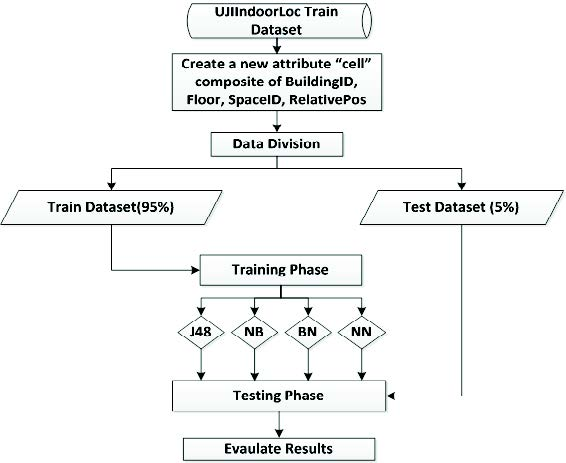
\includegraphics[scale=1]{figures/newattribute.jpg}
%		\caption{The new attribute “cell” construction phase}
%		\label{fig:newAttribute} %% NOTE: always label *after* caption!
%	\end{center}
%\end{figure}

%\todo{Compléter cette partie qui semble importante}

